\section{RAILS analyse} \label{app:railsAnalysis}

\begin{figure}[ht]
    \centering
    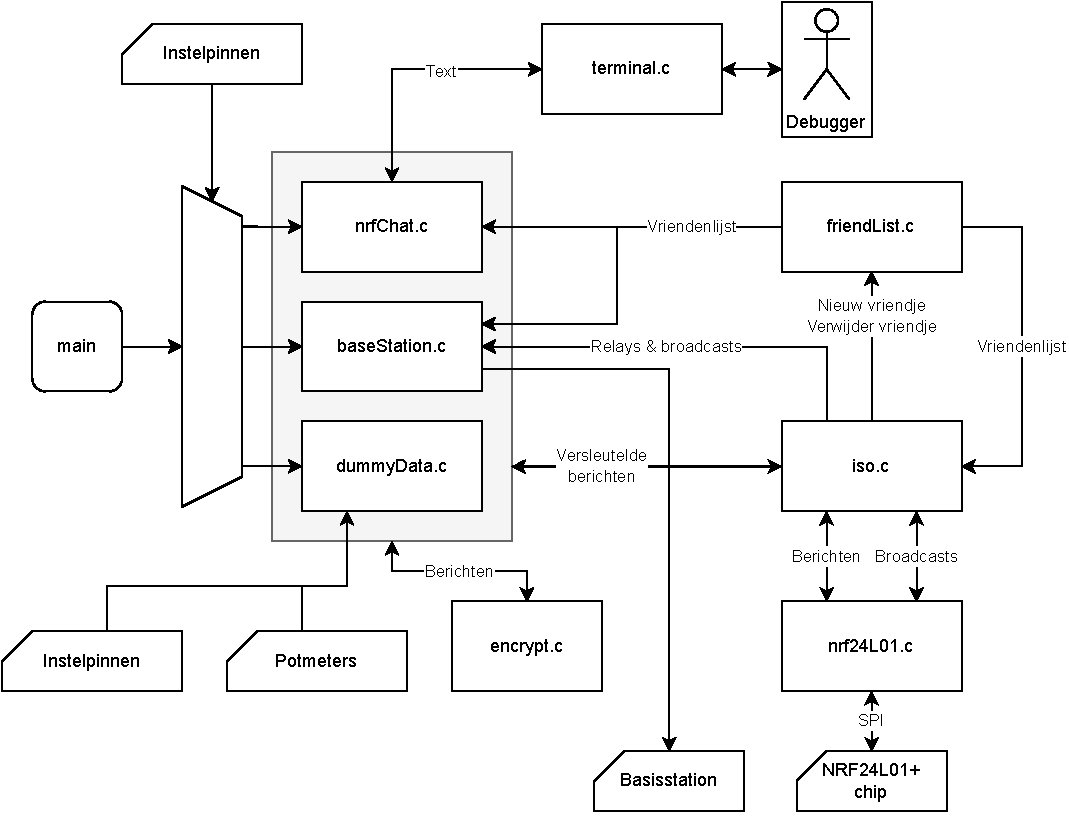
\includegraphics[width=\textwidth]{img/xmegablokshema}
    \caption{Een blokschema van de XMega.}
    \label{fig:xmegaBlokSchema}
\end{figure}

\noindent
In deze analyse zal er worden gekeken naar welke aspecten van de soft/hardware er in de volgende ontwikkel cyclus verbeterd kunnen worden. De analyse methode die wordt gebruikt is de RAILS analyse zoals. Een RAILS analyse bestaat uit de volgende onderdelen:
\begin{itemize}
    \item Revisie
    \item Algoritmes
    \item Interactie
    \item Lookup tabellen
    \item Slaap
\end{itemize}
De bovengenoemde onderdelen zullen in de rest van deze appendix worden beschreven.

\subsection{Revisie}

Voor de revisie is het volledige systeem van de XMega in een blokschema verwerkt. Deze is te zien in \autoref{fig:xmegaBlokSchema}. Het blokschema bevat alle functionele blokken van de code. Deze zijn vanaf het begin van het project al onderverdeeld in aparte C bestanden, waardoor de code erg overzichtelijk is.


\subsection{Algoritmes}

Er is uitgebreid nagedacht over de algoritmes in de code. De belangrijkste algoritmes die het meeste tijd innemen bevinden zich in het iso gedeelte en de vriendenlijst. De vriendenlijst gebruikt een array met zogenaamde `gaten' er in, die ervoor zorgen dat de lijst niet elke keer opgeschoven hoeft te worden wanneer er een vriendje verwijdert wordt. Hier is meer over te lezen in \autoref{sec:vriendjes}.

Een snapshot wordt elke keer dat deze verstuurd wordt opnieuw opgebouwd. Dit is omdat de snapshot maar één keer per seconde gestuurd wordt. Aangezien het netwerk vaak meer dan één node bevat, zullen snapshots een stuk vaker ontvangen dan verzonden worden. Hierdoor zou het continu bijhouden van de snapshot die verstuurd moet worden, terwijl ook de vriendenlijst bijgehouden wordt, kwa snelheid nadelig zijn.

Wanneer er een vriendje toe wordt gevoegd aan de lijst start het algoritme altijd met zoeken bij het begin van de array. Hier is ruimte voor een kleine optimalisatie. Als continu de laagste lege index bijgehouden wordt, (deze zou bijgewerkt worden wanneer er een vriendje verwijdert wordt) hoeft het algoritme niet elke keer door de volledige array. Dit zou niet veel schelen, maar het is toch net iets efficiënter.


\subsection{Interactie}

\subsection{Lookup tabellen}

Aangezien de vriendjes worden opgeslagen in een array die groot genoeg is om het maximum aantal vriendjes op te kunnen slaan, zou het voor de hand liggen om hier ook een lookup tabel voor te gebruiken. De vriendjes kunnen dan op de index van hun ID opgeslagen worden.
\begin{table}[ht]
    \centering
    \begin{tabular}{c|cc}
    Operatie                    & Snelheid nu & Snelheid met lookup tabel \\
    \hline \hline
    Vriendje toevoegen          & \makecell{$O(s)$ \\ $\Theta(n)$ \\ $\Omega(1)$} & \makecell{$O(1)$ \\ $\Theta(1)$ \\ $\Omega(1)$} \\
    \hline
    Vriendje verwijderen        & \makecell{$O(1)$ \\ $\Theta(1)$ \\ $\Omega(1)$} & \makecell{$O(1)$ \\ $\Theta(1)$ \\ $\Omega(1)$} \\
    \hline
    Vriendje vinden in lijst    & \makecell{$O(s)$ \\ $\Theta(n)$ \\ $\Omega(1)$} & \makecell{$O(1)$ \\ $\Theta(1)$ \\ $\Omega(1)$} \\
    \hline
    Door hele lijst heen gaan   & \makecell{$O(s)$ \\ $\Theta(n)$ \\ $\Omega(n)$} & \makecell{$O(s)$ \\ $\Theta(s)$ \\ $\Omega(n)$} \\
    \hline
    \end{tabular}
    \caption{De big O, big $\Theta$ en big $\Omega$ snelheid van de operaties die over de vriendjeslijst worden uitgevoerd. `n' is hier het aantal bekende vriendjes, `s' is de grootte van de array.}
    \label{tab:speedOfTheFriends}
\end{table}

De asymptotische snelheid van de operaties is genoteerd in \autoref{tab:speedOfTheFriends}. Hier is te zien dat, wanneer vriendjes worden opgeslagen op de index van hun ID, dat het algoritme bijna altijd sneller is. De enige situatie waarin dit trager is, is wanneer er door de volledige array heen wordt gezocht. Deze operatie gebeurt een enkele keer wanneer er een snapshot ontvangen wordt, en een enkele keer wanneer er een snapshot opgebouwd wordt. De andere operaties gebeuren veel vaker. Het is dus aan te raden om de vriendjes op te slaan op de index van hun ID.

\subsection{Slaap}
% \fbox{
%     \centering
%     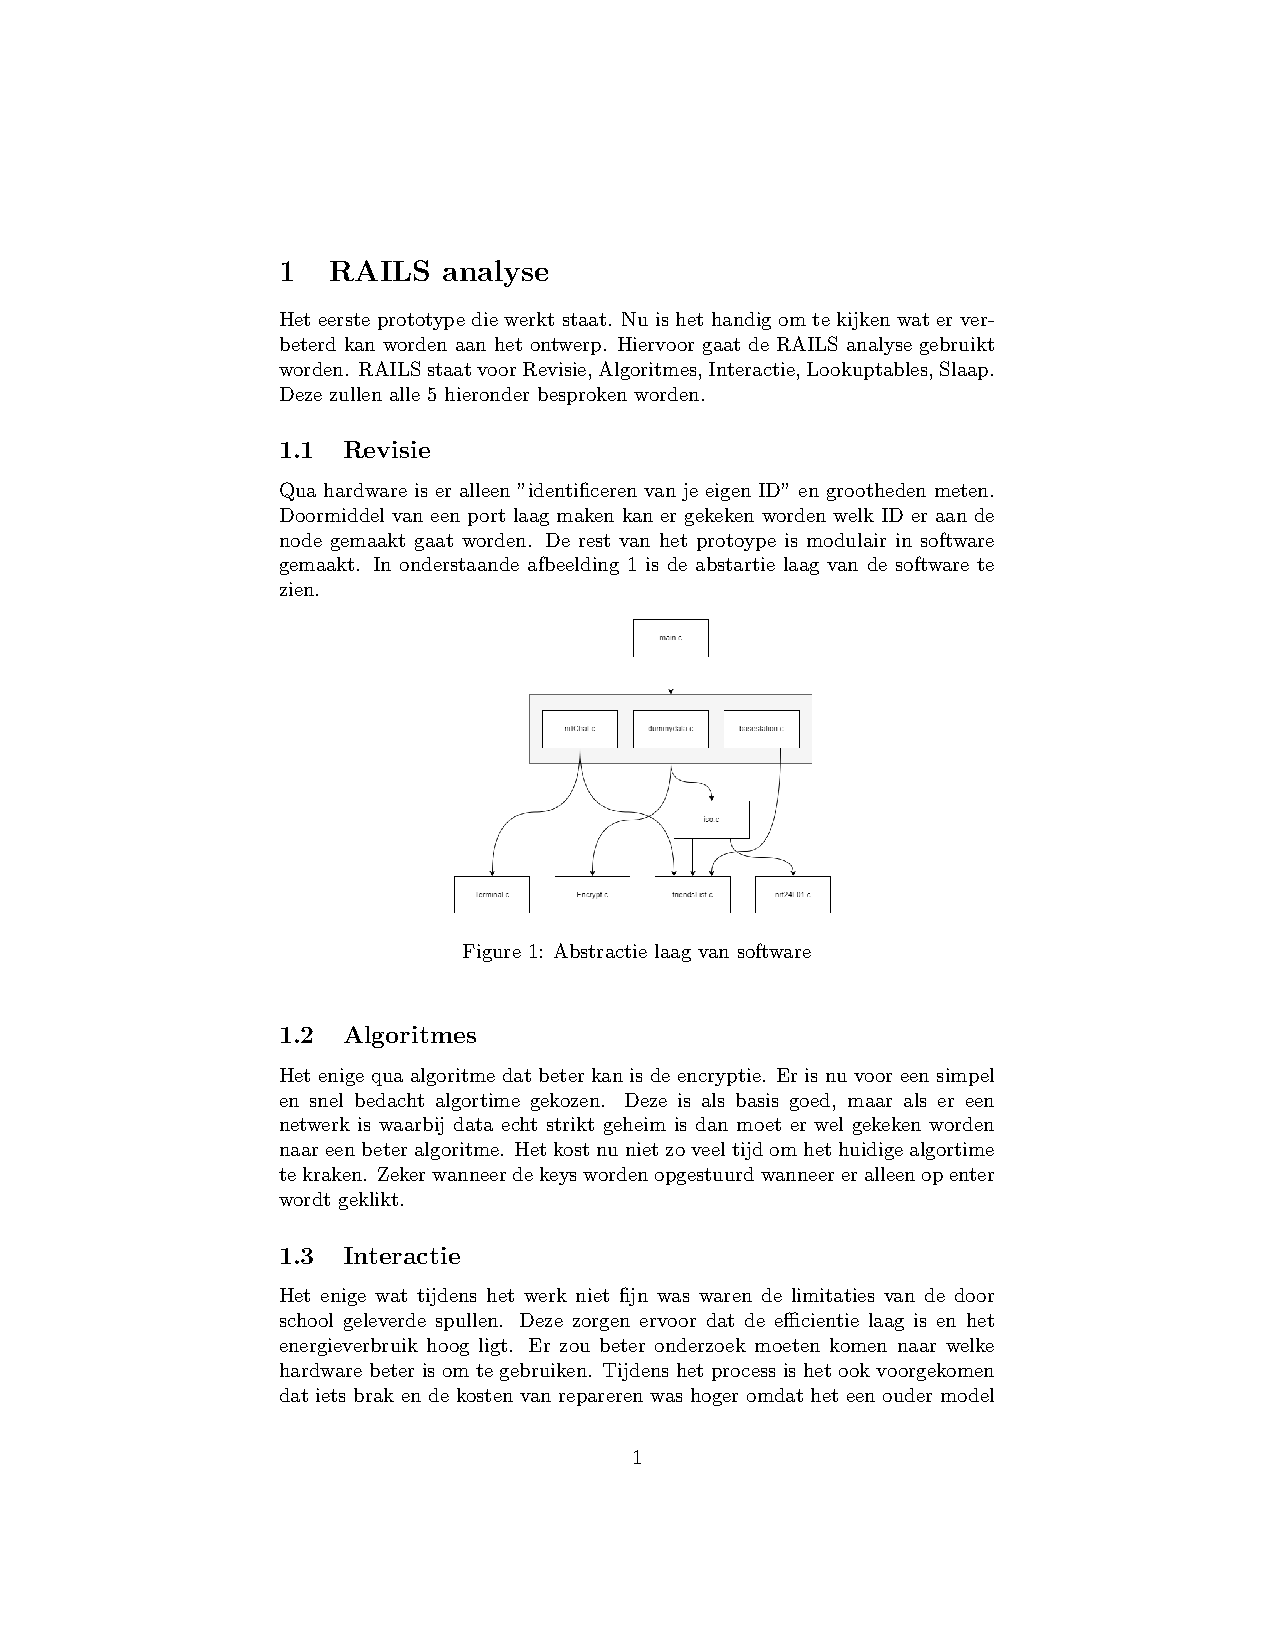
\includegraphics[page=1,scale=0.7]{img/RAILS.pdf}
% }

% \fbox{
%     \centering
%     \includegraphics[page=2,scale=0.7]{img/RAILS.pdf}
% }